\documentclass{beamer}
\usepackage[utf8]{inputenc}

\usetheme{Madrid}
\usecolortheme{default}
\usepackage{amsmath,amssymb,amsfonts,amsthm}
\usepackage{txfonts}
\usepackage{tkz-euclide}
\usepackage{listings}
\usepackage{adjustbox}
\usepackage{array}
\usepackage{tabularx}
\usepackage{gvv}
\usepackage{lmodern}
\usepackage{circuitikz}
\usepackage{tikz}
\usepackage{graphicx}

\setbeamertemplate{page number in head/foot}[totalframenumber]

\usepackage{tcolorbox}
\tcbuselibrary{minted,breakable,xparse,skins}



\definecolor{bg}{gray}{0.95}
\DeclareTCBListing{mintedbox}{O{}m!O{}}{%
  breakable=true,
  listing engine=minted,
  listing only,
  minted language=#2,
  minted style=default,
  minted options={%
    linenos,
    gobble=0,
    breaklines=true,
    breakafter=,,
    fontsize=\small,
    numbersep=8pt,
    #1},
  boxsep=0pt,
  left skip=0pt,
  right skip=0pt,
  left=25pt,
  right=0pt,
  top=3pt,
  bottom=3pt,
  arc=5pt,
  leftrule=0pt,
  rightrule=0pt,
  bottomrule=2pt,
  toprule=2pt,
  colback=bg,
  colframe=orange!70,
  enhanced,
  overlay={%
    \begin{tcbclipinterior}
    \fill[orange!20!white] (frame.south west) rectangle ([xshift=20pt]frame.north west);
    \end{tcbclipinterior}},
  #3,
}
\lstset{
    language=C,
    basicstyle=\ttfamily\small,
    keywordstyle=\color{blue},
    stringstyle=\color{orange},
    commentstyle=\color{green!60!black},
    numbers=left,
    numberstyle=\tiny\color{gray},
    breaklines=true,
    showstringspaces=false,
}
%------------------------------------------------------------
%This block of code defines the information to appear in the
%Title page
\title %optional
{1.9.32}
\date{August 30,2025}
%\subtitle{A short story}

\author % (optional)
{Sai Hasini Pappula-EE25BTECH11044}

\begin{document}

%-------------------------------------------------
\begin{frame}{Question}
\begin{block}{Problem}
If the distance between the points $(3,-5)$ and $(x,-5)$ is $15$ units, then find the values of $x$ using matrices.
\end{block}
\end{frame}

%-------------------------------------------------
\begin{frame}{Solution Process}
\textbf{Step 1: Represent points}\\[4pt]
\[
\vec{A} = \begin{bmatrix} 3 \\ -5 \end{bmatrix}, 
\quad 
\vec{B} = \begin{bmatrix} x \\ -5 \end{bmatrix}
\]

\textbf{Step 2: Distance formula using matrices}\\[4pt]
\[
d^2 = (\vec{B}-\vec{A})^T(\vec{B}-\vec{A})
\]

\textbf{Step 3: Substitution}\\[4pt]
\[
d^2 = \begin{bmatrix} x-3 \\ 0 \end{bmatrix}^T 
       \begin{bmatrix} x-3 \\ 0 \end{bmatrix} 
     = (x-3)^2
\]
\end{frame}

%-------------------------------------------------
\begin{frame}{Final Answer}
Given $d=15$, we get
\[
(x-3)^2 = 225
\]
\[
x-3 = \pm 15
\]
\[
\therefore \quad x = 18 \quad \text{or} \quad x = -12
\]
\end{frame}

%-------------------------------------------------
\begin{frame}[fragile]{C Code}
\begin{lstlisting}[language=C]
#include <stdio.h>
#include <math.h>

// Distance formula
double distance(double A[2], double B[2]) {
    return sqrt((B[0]-A[0])*(B[0]-A[0]) +
                (B[1]-A[1])*(B[1]-A[1]));
}

int main() {
    double A[2] = {3, -5};
    double B[2];
    double d;

    printf("Enter x-coordinate of B: ");
    scanf("%lf", &B[0]);
    B[1] = -5;

    d = distance(A, B);

    printf("Distance = %.2f\n", d);
    return 0;
}
\end{lstlisting}
\end{frame}

%-------------------------------------------------
\begin{frame}[fragile]{Python Code (1/2)}
\begin{lstlisting}[language=Python]
import matplotlib.pyplot as plt

# Given point
A = (3, -5)
d = 15  # distance

# Solve for x
x1 = 18
x2 = -12

B1 = (x1, -5)
B2 = (x2, -5)

print("Solutions for x:", x1, "and", x2)
\end{lstlisting}
\end{frame}

%-------------------------------------------------
\begin{frame}[fragile]{Python Code (2/2 - Plotting)}
\begin{lstlisting}[language=Python]
plt.figure(figsize=(8,6))
plt.axhline(0, color='black')
plt.axvline(0, color='black')

# Plot points
plt.scatter(*A, color='black', s=80)
plt.text(A[0]+0.3, A[1]+0.5, "A(3,-5)")

plt.scatter(*B1, color='blue', s=80)
plt.text(B1[0]+0.3, B1[1]+0.5, "B1(18,-5)")

plt.scatter(*B2, color='red', s=80)
plt.text(B2[0]+0.3, B2[1]+0.5, "B2(-12,-5)")

# Plot lines
plt.plot([A[0], B1[0]], [A[1], B1[1]], 'b-', lw=2, label="15 units")
plt.plot([A[0], B2[0]], [A[1], B2[1]], 'r--', lw=2, label="15 units")

plt.legend()
plt.show()
\end{lstlisting}
\end{frame}

%-------------------------------------------------
\begin{frame}{Graphical Representation}
\begin{center}
 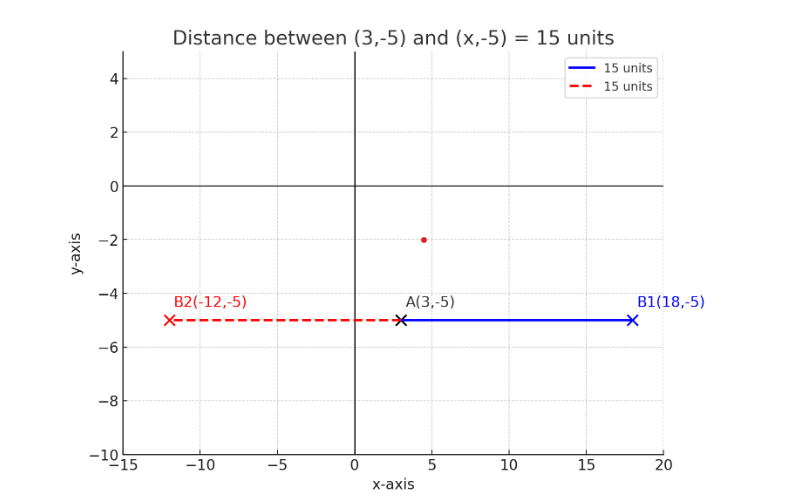
\includegraphics[width=0.6\columnwidth]{figs/plot2.png}
\end{center}
\end{frame}

\end{document}
